
\subsection{Classifying BLT-Sets}


We will describe one application that falls in the area of finite geometry. 
A $Q(4,q)$ space is a four-dimensional projective space over the field $\bbF_q$ equipped with a non-degenerate quadratic form. 
In such a space, sets of points that are known as BLT-sets are of interest.
A BLT-set is a set of $q+1$ points on the $Q(4,q)$ quadric 
satisfying a triple condition. 
Namely, whenever $P,Q,R$ are any three points of the BLT-set then $(P+Q+R)^\perp$ 
is an anisotropic line. This means that the three points form a triad 
(a triangle without any sides) such that no point of $Q(4,q)$ 
is  collinear to all three of $P,Q,R$.
BLT-sets are known to exist whenever $q$ is an odd prime power. 
It is an important problem to classify BLT-sets. 
By this, we mean the following: Two BLT-sets of $Q(4,q)$ are isomorphic 
if there is a collineation of $Q(4,q)$ that takes one set to the other. 
The classification problem for BLT-sets asks for the isomorphism classes of BLT-sets. 
This is computing the orbits of the group of collineations on 
the set of BLT-sets of $Q(4,q).$



\bigskip

To classify BLT-sets of $Q(4,q)$ using \verb'orbiter', 
we again use the principle of 
Breaking the Symmetry. In this case, this means 
we will classify partial BLT-sets of size $s$ first, where $s$ is a relatively small number (compared to $q$). 
The representative of these orbits are the starter. 
Once this is done, 
all BLT-sets containing any of the starter will be computed. 
This is done using rainbow cliques in colored graphs. 
Finally, another round 
of isomorph classification will take place. 
Once all this is done, we can create a pdf file containing the classification
in human-readable format.


\bigskip


The main program that we use is called \verb'blt.out'. It resides in 
\begin{quote}
\verb'ORBITER/SRC/APPS/BLT'\\
\end{quote}
and facilitates the search 
and classification for BLT-sets and partial BLT-sets. 
Here, a partial BLT-set is a set of points on the $Q(4,q)$ quadric such that 
$(P+Q+R)^\perp$ 
is an anisotropic line for any three points $P,Q,R$ in the set.
Thus, a BLT-set is a partial BLT-set of size $q+1.$
For small values of $q$, one can classify the BLT-sets using \verb'blt.out'.
The search tree for the BLT sets in $Q(4,11)$ has $189$ nodes and looks like this:
$$
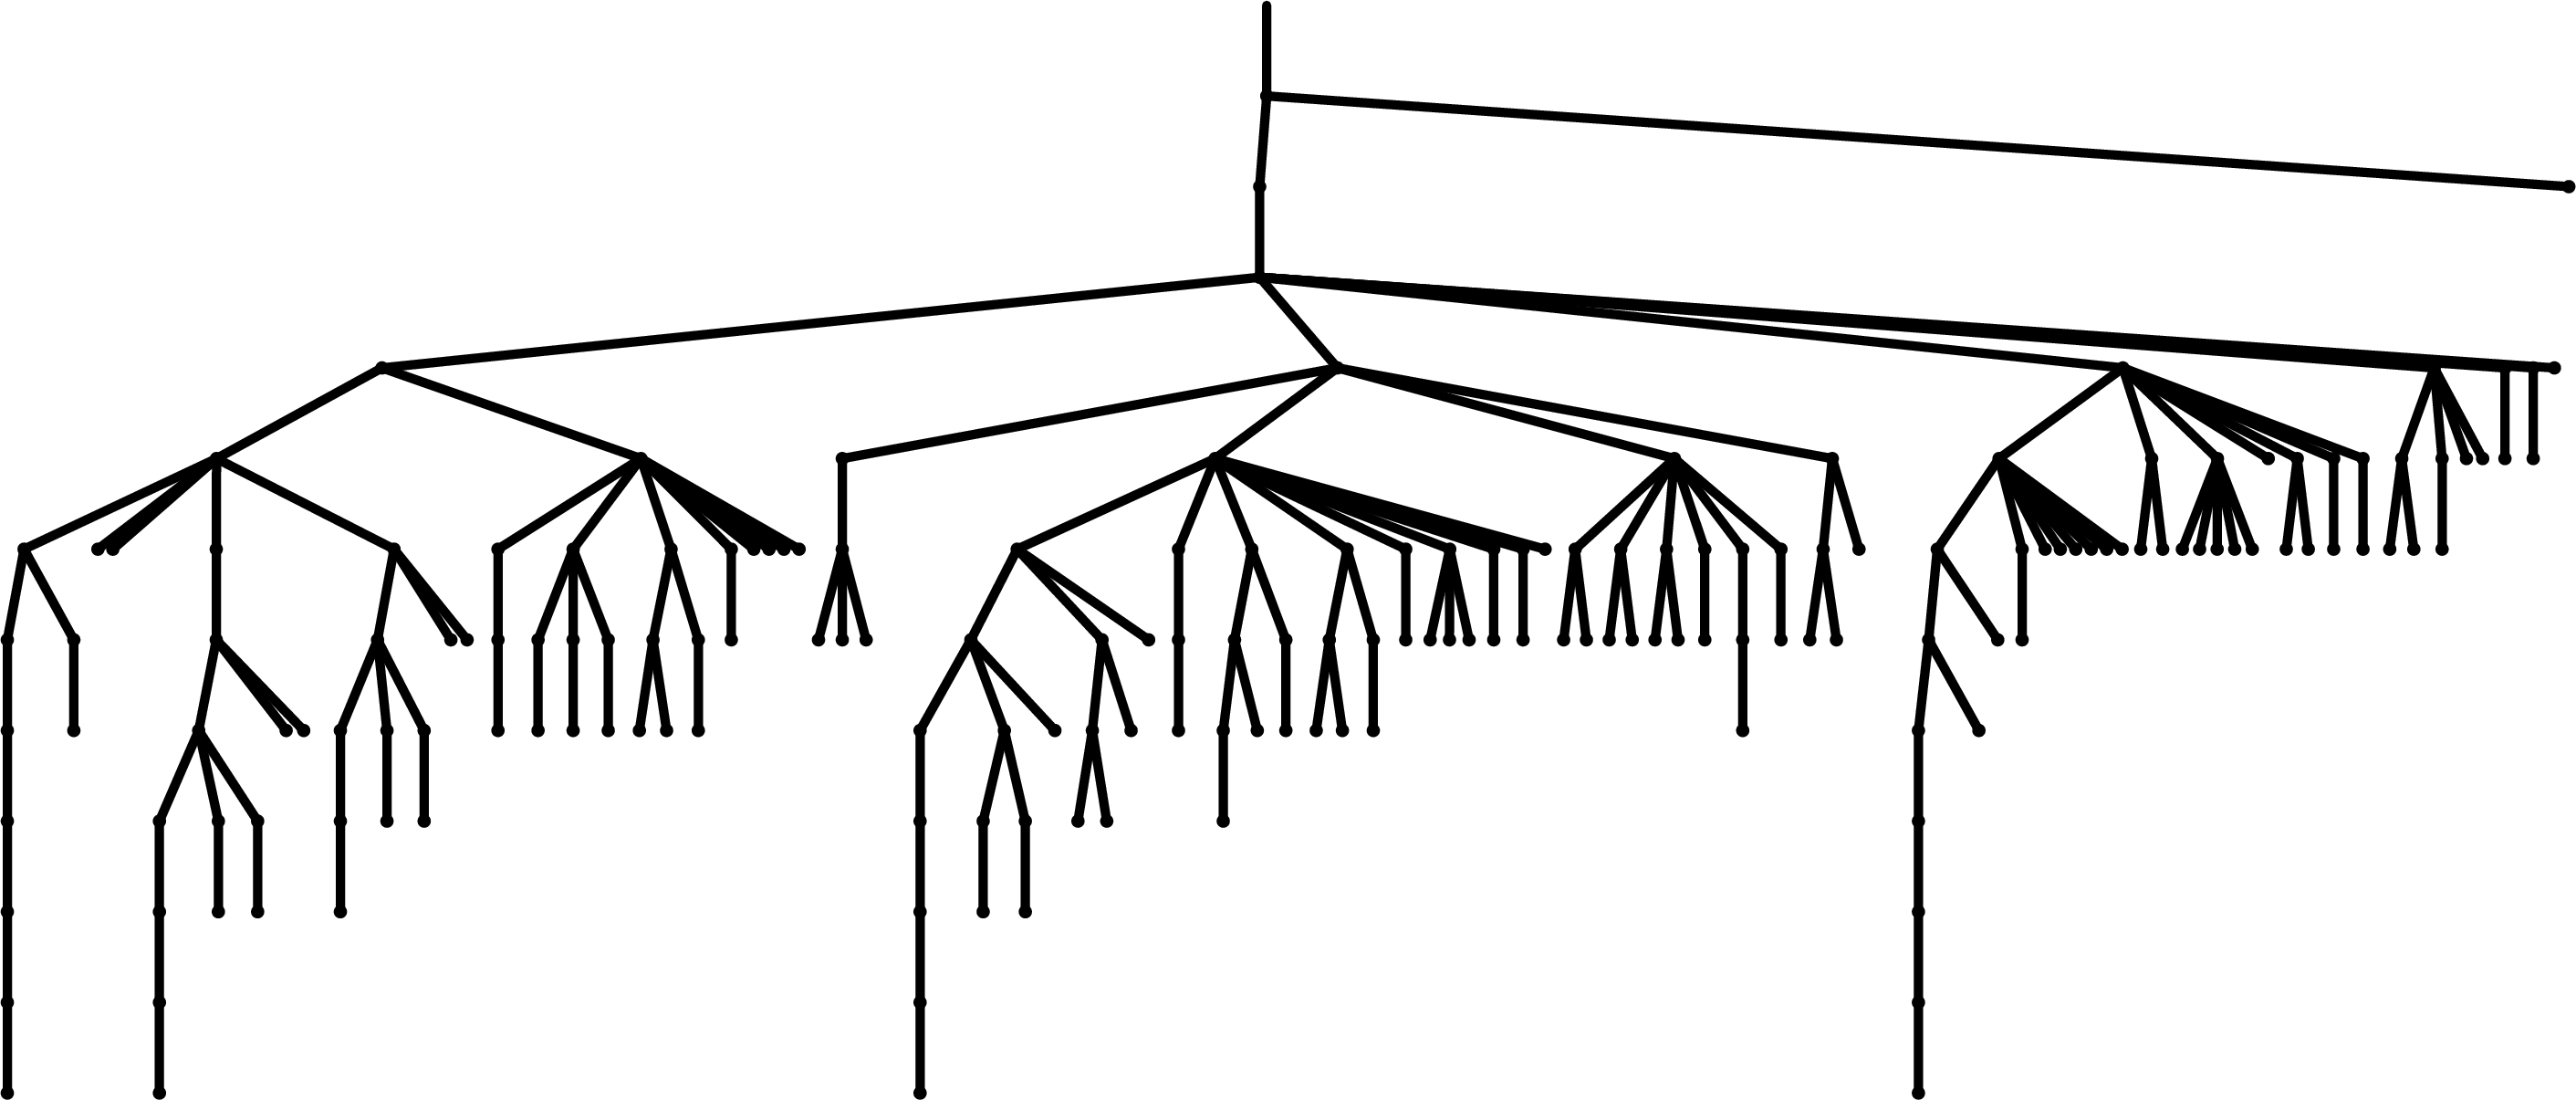
\includegraphics[width=150mm]{GRAPHICS/BLT_11_tree}
$$
The four isomorphism classes of BLT-sets of $Q(4,11)$ correspond 
to the leaves at depth $12$ in this tree.



\bigskip




The program \verb'blt.out' relies on the class \verb'blt_generator' in 
\begin{quote}
\verb'ORBITER/SRC/APPS/BLT/blt_generator.C'
\end{quote}
The class \verb'blt_generator' maintains the quadric $Q(4,q)$ 
together with its group $\PGGO(5,q).$
The incidence structure of the quadric is encoded in an object 
\begin{quote}
\verb'orthogonal *O;'
\end{quote}
The object \verb'O' is set up automatically by the function that sets up the group, 
which is
\begin{quote} 
\verb'A->init_orthogonal_group(epsilon, n, q, override_poly,' \\
\verb'    f_semilinear, f_basis, 0/*verbose_level - 2*/);'\\
\end{quote}
Here, \verb'A' is an action object that is part of the class \verb'arc_generator', 
\verb'epsilon' is $0$, \verb'n' is $4$, and \verb'q' is the field order. 
The argument \verb'override_poly' is a number 
specifying a polynomial over $\bbF_p$ that 
is used to create the field $\bbF_q$ 
(this is only relevant if $q=p^h$ for some prime $p$ 
and some integer $h > 1$).
The flag \verb'f_semilinear' specifies if we want the semilinear group 
and the flag \verb'f_basis' specifies if we want to set up a stabilizer chain 
for the group (it should be \verb'TRUE').
Once the orthogonal group is set up, we can initialize two object pointers:
\begin{quote}
\verb'matrix_group *M;'\\
\verb'orthogonal *O;'\\
\verb'M = A->subaction->G.matrix_grp;'\\
\verb'O = M->O;'\\
\end{quote}

\bigskip


